\section{Suite de la séance 15 (séance 16)}

\begin{theorement}{}
    \textbf{Sur $\C$ :} Soit $A \in \mathcal{M}_n(\C)$. $\Sim_{\C}(A) = \{ P A P^{-1} \mid P \in GL_n(\C) \}$ est fermé $\iff A$ diagonalisable sur $\C$.
    
    \lvspace
    \textbf{Sur $\R$ :} Soit $A \in \mathcal{M}_n(\R)$. $\Sim_{\R}(A)$ est fermé dans $\mathcal{M}_n(\R) \iff A$ diagonalisable sur $\C$.
\end{theorement}

\begin{proof}
    \uindent{Sur $\C$}
    
    $\implies$ On suppose $A$ diagonalisable. Soit $(M_k) \in (\Sim_{\C}(A))^\N$ telle que $M_k \to M$.
    Pour tout $k$, on a $M_k \sim A$, donc $\chi_{M_k} = \chi_A$.
    Le passage à la limite $k \to +\infty$ donne $\chi_M = \chi_A$ car l'application $N \mapsto \chi_N$ est continue.

    \skull \textbf{Danger :} L'application $N \mapsto \pi_N$ (polynôme minimal) n'est pas continue.
    On peut le voir avec le contre-exemple : $\begin{pmatrix} 1 & \varepsilon \\ 0 & 1 \end{pmatrix}$.

    Cependant, on a $\pi_A(A) = 0$ donc $\pi_A(M_k) = 0$. En revanche, l'application $N \mapsto \pi_A(N)$ est, elle, continue.
    Donc par passage à la limite, $\pi_A(M) = 0$.
    Comme $A$ est diagonalisable, $\pi_A$ est scindé à racines simples. Le fait que $\pi_A(M) = 0$ implique donc que $M$ est diagonalisable.

    De plus $\chi_M = \chi_A$, et $A$ est diagonalisable.
    Donc $A$ et $M$ ont le même spectre, avec les mêmes multiplicités.
    Ils sont donc semblables à la même matrice diagonale, ce qui implique que $M \in \Sim_{\C}(A)$.

    \lvspace
    $\impliedby$ On suppose $\Sim_{\C}(A)$ fermé. En se plaçant sur $\C$, on peut trigonaliser $A$ : il existe $P \in GL_n(\C)$ tel que $A = P T P^{-1}$.
    Soit la matrice diagonale $D_\varepsilon = \text{diag}(1, \varepsilon, \dots, \varepsilon^{n-1})$.
    On a :
    \[
    D_\varepsilon^{-1} T D_\varepsilon = \begin{pmatrix} t_{11} & \varepsilon t_{12} & \dots \\ 0 & \ddots & \vdots \\ 0 & 0 & t_{nn} \end{pmatrix} \xrightarrow{\varepsilon \to 0} \begin{pmatrix} t_{11} & & 0 \\ & \ddots & \\ 0 & & t_{nn} \end{pmatrix} = D
    \]
    On a construit une suite de matrices semblables à $A$ qui converge vers $D$, donc $D \in \overline{\Sim_{\C}(A)}$. 
    Or $\Sim_{\C}(A)$ est fermé, donc $D \in \Sim_{\C}(A)$.
    Ainsi, il existe $P \in GL_n(\C)$ tel que $A = P D P^{-1}$ et donc $A$ est diagonalisable.

    \lvspace
    \uindent{Sur $\R$}
    
    \begin{remarque}
        On a $\Sim_{\R}(A) = \Sim_{\C}(A) \cap \mathcal{M}_n(\R)$.
        Pour le montrer : on écrit $A = P B P^{-1}$, puis $P^{-1}A = B P^{-1}$. On pose un paramètre et on sépare les parties réelles et imaginaires. On trouve alors une matrice de passage réelle.
    \end{remarque}

    $\impliedby$ Si $A$ est diagonalisable sur $\C$, $\Sim_{\C}(A)$ est fermé. De plus, $\mathcal{M}_n(\R)$ est fermé dans $\mathcal{M}_n(\C)$.
    Donc $\Sim_{\R}(A)$ est fermé en tant qu'intersection de fermés.

    \lvspace
    $\implies$ 
    \textbf{Cas $n=2$ :} disjoint du cas où l'endomorphisme possède 1 ou 2 valeurs propres réelles, et on a le même type d'arguments que sur $\C$.
    
    \textbf{Cas $n \ge 3$ :} on utilise la décomposition de Jordan sur $\R$.     Soit $M \in \mathcal{M}_n(\R)$. On a :
    \[
    M \sim_{\R} \begin{pmatrix} J_{\lambda_1} & & 0 \\ & \ddots & \\ 0 & & J_{r_k} \end{pmatrix} \quad \text{avec} \quad J_\lambda(1) = \begin{pmatrix} \lambda & 1 & 0 \\ & \ddots & 1 \\ 0 & & \lambda \end{pmatrix}
    \]
    Plus précisément, $M \sim \begin{pmatrix} J_{\mu_1}(n_1) & & 0 \\ & \ddots & \\ 0 & & J_{\lambda_i}(n_i) \end{pmatrix} \implies \mu_i \in \R \text{ et } \lambda_i \in \C$.
    
    Notons $\lambda_1 = a_1 + i b_1$. Pour le bloc complexe, on a l'équivalence :
    \[
    \begin{pmatrix} J_{\lambda_1}(n_1) & 0 \\ 0 & J_{\bar{\lambda}_1}(n_1) \end{pmatrix} \sim \begin{pmatrix} \begin{pmatrix} a_1 & -b_1 \\ b_1 & a_1 \end{pmatrix} & I_2 & 0 \\ & \ddots & \ddots \\ 0 & & \begin{pmatrix} a_1 & -b_1 \\ b_1 & a_1 \end{pmatrix} \end{pmatrix}
    \]
    Et donc, sur les réels :
    \[
    M \sim_{\R} \begin{pmatrix} \begin{pmatrix} a_1 & -b_1 \\ b_1 & a_1 \end{pmatrix} & I_2 & 0 \\ & \ddots & \ddots \\ 0 & & \begin{pmatrix} a_1 & -b_1 \\ b_1 & a_1 \end{pmatrix} \end{pmatrix} = J
    \]
    On a donc $M = P J P^{-1}$. 
    On pose $D_\varepsilon = \text{diag}(I_2, \varepsilon I_2, \dots, \varepsilon^{n-1} I_2)$. Alors :
    \[
    D_\varepsilon^{-1} J D_\varepsilon = \begin{pmatrix} \begin{pmatrix} a_1 & -b_1 \\ b_1 & a_1 \end{pmatrix} & \varepsilon I_2 & 0 \\ & \ddots & \ddots \\ 0 & & \begin{pmatrix} a_1 & -b_1 \\ b_1 & a_1 \end{pmatrix} \end{pmatrix} \xrightarrow{\varepsilon \to 0} D = \begin{pmatrix} \begin{pmatrix} a_1 & -b_1 \\ b_1 & a_1 \end{pmatrix} & & 0 \\ & \ddots & \\ 0 & & \begin{pmatrix} a_1 & -b_1 \\ b_1 & a_1 \end{pmatrix} \end{pmatrix}
    \]
    Et on remarque que $D \sim_{\C} \begin{pmatrix} \lambda_1 & & 0 \\ & \ddots & \\ 0 & & \bar{\lambda}_1 \end{pmatrix} \in \overline{\Sim_{\R}(M)}$.
\end{proof}

\section{Calcul différentiel}

\begin{theorement}{}
    Soit $K \subset \R^n$, avec $K$ compact.
    Soit $h : K \to K$ telle que $\forall x \neq y, \ \norm{h(x) - h(y)} < \norm{x - y}$.
    $\implies h$ possède un unique point fixe.
\end{theorement}

\begin{proof}
    L'application $\fonction{f}{K}{\R^+}{x}{\norm{h(x) - x}}$ est continue sur $K$ compact.
    Donc par le théorème des bornes atteintes, $\exists a \in K$ tel que $\norm{h(a) - a} = \min_{x \in K} \norm{h(x) - x}$.
    
    Si $h(a) \neq a$ :
    \[
    \norm{h(h(a)) - h(a)} < \norm{h(a) - a}
    \]
    Ceci est en contradiction avec la minimalité en $a$. 
    Donc $h(a) = a$.
\end{proof}

\begin{theoreme}{Application du théorème d'inversion locale}{}
    Soit $f : \R^n \to \R^n$ de classe $\mc{1}$ telle que :
    \begin{enumerate}
        \item $A = \{x \in \R^n \mid df(x) \notin GL_n(\R)\}$ est fini.
        \item $\norm{f(x)} \tpinf{\norm{x}} +\infty$.
    \end{enumerate}
    Alors $f$ est surjective.
\end{theoreme}

\begin{theoreme}{Application : d'Alembert-Gauss}{}
    Soit $P : \C \to \C$ un polynôme non constant.
    Alors $P$ possède une racine (i.e. $P$ est surjectif).
\end{theoreme}

\begin{proof}
    On vérifie facilement la coercivité : $\abs{P(z)} \tpinf{\abs{z}} +\infty$.
    On peut voir le polynôme comme $P : \C \to \C, z \mapsto P(z)$ ou comme une application vectorielle $\tilde{P} : \R^2 \to \R^2, (x,y) \mapsto P(x,y)$.
    Soit $z \in \C$, on note $P'(z) = a + i b$.
    La différentielle s'écrit $d\tilde{P}(x,y) = \begin{pmatrix} a & -b \\ b & a \end{pmatrix}$.
    Et on a $\det(d\tilde{P}) = a^2 + b^2 = \abs{P'(z)}^2$.
    L'ensemble $\{z \in \C \mid P'(z) = 0\}$ est bien fini car $P'$ est un polynôme.

    \lvspace
    \emph{Démo du théorème de surjectivité :}
    
    Soit $A = \{x \in \R^n \mid df(x) \notin GL_n(\R)\}$. L'ensemble $B = f(A)$ est un ensemble fini.
    $\Omega_2 = \R^n \setminus B$ est un ouvert, et est connexe par arcs (vrai car $n \ge 2$).

    \begin{center}
    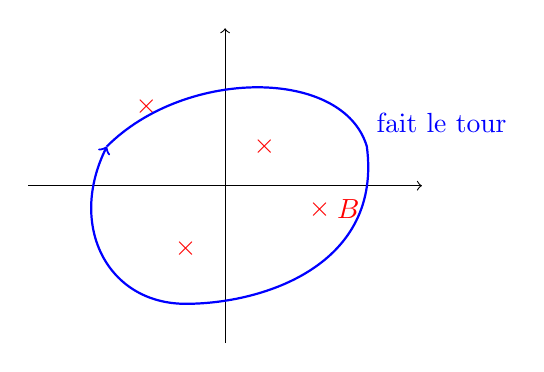
\begin{tikzpicture}[scale=1]
        \draw[->] (-2.5,0) -- (2.5,0);
        \draw[->] (0,-2) -- (0,2);
        
        % Points de l'ensemble B
        \node[red] at (0.5, 0.5) {$\times$};
        \node[red] at (-0.5, -0.8) {$\times$};
        \node[red] at (1.2, -0.3) {$\times$};
        \node[red] at (-1, 1) {$\times$};
        \node[red, right] at (1.3, -0.3) {$B$};
        
        % Chemin qui fait le tour
        \draw[->, blue, thick] (-1.5, 0.5) .. controls (-0.5, 1.5) and (1.5, 1.5) .. (1.8, 0.5) .. controls (2, -1) and (0.5, -1.5) .. (-0.5, -1.5) .. controls (-1.5, -1.5) and (-2, -0.5) .. (-1.5, 0.5);
        \node[blue, right] at (1.8, 0.8) {fait le tour};
    \end{tikzpicture}
    \end{center}

    Soit $\Omega_1 = f^{-1}(\Omega_2) = \{x \in \R^n \mid f(x) \in \Omega_2\}$.
    On considère la restriction $f_{|\Omega_1} : \Omega_1 \to \Omega_2$.

    \uindent{Affirmation} $f_{|\Omega_1} : \Omega_1 \to \Omega_2$ est surjective.
    On veut montrer que $f(\Omega_1)$ est à la fois ouvert et fermé dans $\Omega_2$, ce qui impliquera par connexité que $f(\Omega_1) = \Omega_2$.

    \textbf{1. $f(\Omega_1)$ est ouvert :}
    Soit $x \in \Omega_1$. Par définition, on a $df(x) \in GL_n(\R)$.
    Par le théorème d'inversion locale, il existe un ouvert $V$ contenant $x$ tel que $f(V)$ soit ouvert.

    \begin{center}
    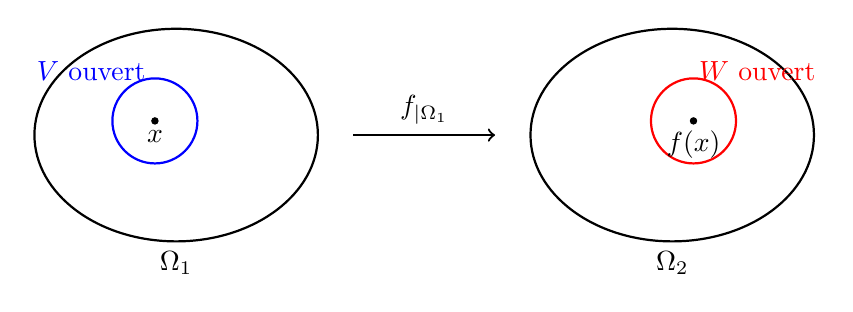
\begin{tikzpicture}[scale=0.9]
        % Espace de départ
        \draw[thick] (0,0) ellipse (2 and 1.5);
        \node at (0, -1.8) {$\Omega_1$};
        
        \draw[blue, thick] (-0.3, 0.2) circle (0.6);
        \fill (-0.3, 0.2) circle (1.5pt) node[below] {$x$};
        \node[blue] at (-1.2, 0.9) {$V$ ouvert};

        % Flèche de l'application
        \draw[->, thick] (2.5, 0) -- (4.5, 0) node[midway, above] {$f_{|\Omega_1}$};

        % Espace d'arrivée
        \draw[thick] (7,0) ellipse (2 and 1.5);
        \node at (7, -1.8) {$\Omega_2$};
        
        \draw[red, thick] (7.3, 0.2) circle (0.6);
        \fill (7.3, 0.2) circle (1.5pt) node[below] {$f(x)$};
        \node[red] at (8.2, 0.9) {$W$ ouvert};
    \end{tikzpicture}
    \end{center}

    On a $x \in V \subset \Omega_1$ et $f(x) \in W = f(V) \subset f(\Omega_1)$.
    Comme ceci est vrai pour tout $x \in \Omega_1$, $f(\Omega_1)$ est bien un ouvert.

    \textbf{2. $f(\Omega_1)$ est fermé dans $\Omega_2$ :}
    Soit $(y_m) \in (f(\Omega_1))^\N$ une suite convergeant vers $y \in \Omega_2$, avec $y_m = f(x_m)$ où $x_m \in \Omega_1$.
    La suite $(y_m)$ est convergente donc bornée, ce qui implique que la suite $(x_m)$ est également bornée (d'après l'hypothèse 2 de coercivité).
    Par le théorème de Bolzano-Weierstrass, il existe une sous-suite $x_{\varphi(m)}$ qui converge vers une limite $x$.
    Par continuité de $f$, on a $f(x_{\varphi(m)}) \to f(x)$.
    Or, on sait que $y_{\varphi(m)} \to y \in \Omega_2$. Par unicité de la limite, $y = f(x)$.
    Comme $x \in \Omega_1$, on a $f(x) \in f(\Omega_1)$, ce qui montre que $f(\Omega_1)$ est fermé dans $\Omega_2$.

    \lvspace
    \textbf{Conclusion :}
    Comme $\Omega_2$ est connexe par arcs et que $f(\Omega_1)$ est un sous-ensemble non vide, ouvert et fermé dans $\Omega_2$, on a nécessairement $f(\Omega_1) = \Omega_2$.
    
    Soit $y \in \R^n = B \cup \Omega_2$. 
    Si $y \in \Omega_2$, il possède un antécédent dans $\Omega_1$. Si $y \in B$, il possède un antécédent dans $A$ par définition. 
    Donc tout $y \in \R^n$ possède un antécédent, l'application est surjective.
\end{proof}